\documentclass{article}

\usepackage[utf8]{inputenc}
\usepackage[ngerman]{babel}
\usepackage[T1]{fontenc}
\usepackage{enumitem}
\usepackage{graphicx}
\usepackage{float}

\newlist{FA}{enumerate}{1}
\setlist[FA]{label=/FA\arabic*/}

\newlist{NA}{enumerate}{1}
\setlist[NA]{label=/NA\arabic*/}


\title{Cryptographics Pflichtenheft}
\author{}
\date{\today}

\begin{document}

\maketitle
\tableofcontents
\newpage

\section{Zielbestimmung}
Im Rahmen der PSE-Veranstaltung soll für das Kryptologikum des Instituts für 
Kryptographie und Sicherheit eine Software (Cryptographics / Anicrypto?) zur 
Demonstration kryptographischer Verfahren erstellt werden. \\
\\
Das Programm soll im Laufe der Ausstellung Kryptologikum das 
Interesse der Besucher wecken, 
sich mit Verschlüsselung zu befassen und 
schließlich auch ausgewählte Inhalte der Kryptographie näher bringen
\\
\\
Soll Spaß machen.

\subsection{Musskriterien}

\begin{itemize}
    \item Implementierung der Caesar-Chiffre
    \item Implementierung Vigen`ere-Chiffre
    \item Implementierung RSA
    \item Implementierung Diffie-Hellmann
    \item Implementierung Hashfunktionen
    \item Robuste Programmierung
    \item Intuitive Benutzerführung
    \item Schnelle Reaktionszeiten
    \item Zugriff auf Krypto-Verfahren über Zeitleiste:
        \begin{itemize}
            \item Pop-Up mit kurzem Umriss des Verfahrens
            \item Draufklicken um zum Verfahren zu Gelangen
            \item Einfärbung grün/gelb/rot nach Komplexität des Verfahrens
        \end{itemize}
    \item Drei Optionen je Verfahren: Demo, Selsbstversuch, weitere Informationen
    \item Angeleiter Selbstversuch bei "roten" Verfahren
    \item Interaktion des Benutzers über den Touchscreen
    \item einfache, übersichtliche UI, die sich gut auf Touchscreen bedienen lässt
    \item Robustheit gegen au"sergewöhnliche Interaktion
    \item Man soll das Programm nicht schlie"sen können währen der Vorführung
    \item Praxisbezug bei modernen Kryptoverfahren
    \item Sammlung wiederverwendbare UI-Element um z.B. die Texteingabe gleich
        zu behandeln
    \item Krypto-Algorithmen lassen sich schrittweise ausführen, um den Prozess
        langsam zu verdeutlichen (bspw. bei Caesar: Buchstabe für Buchstabe
        bis Codewort generiert wurde)
    \item der Benutzer soll die Möglichkeit bekommen Dinge Schritt für Schritt
        in seiner eigenen Geschwindigkeit nachzuvollziehen und ggf.
        zurückspringen können

    \item Es darf kein Zurückkommen zum Betriebssystem möglich sein
    \item Visualisierungen sollten Grafiken und Animationen verwenden um Vorgänge zu verdeutlichen
\end{itemize}

\subsection{Wunschkriterien}

\begin{itemize}
    \item Implementierung Public Key – Infrastruktur
    \item Implementierung Shamir Secret Sharing
    \item Implementierung Passwortsicherheit
    \item Implementierung One-Time-Pad
    \item Implementierung Blockchiffre (DES, AES)
    \item Bei Problemen im Selbstversuch hilft der Computer mit Tipps aus
    \item Modulares Austauschen/Hinzufügen von weiteren kryptografischen Verfahren
    \item Einschätzung des aktuellen Wissenstands des Benutzers.
    \item Implementierung elliptischer Kurven
    \item Literaturhinweise(auch weiterführende Literatur), sofern Interesse besteht.
    \item Visualisierungen sollten möglichst ansprechend sein, indem sie z.B. Analogien 
        verwenden (ein Datenpaket wird zu einer Postkarte, ein Schlüssel wird zum einem tatsächlichen Schlüssel, ...).
    \item Wenn über einen Zeitraum x keine Nutzereingaben erfolgen erscheint ein Countdown 
        nach dessen Ablauf das Programm auf den Willkommensbildschirm zurücksetzt
    \item Visualisierung von Modulo mit einer Uhr
    \item Visualisierung von Angriffen auf Verfahren
    \item (Blockchiffre im ECB-Modus vs. CBC-Modus, siehe Bild in 
    \item http://de.wikipedia.org/wiki/Electronic\_Code\_Book\_Mode)
    \item Brute-Force Angriff auf (symmetrisch/asymmetrisch?) Verschlüsselung
    \item Enigma?
    \item Zahlentheorie: modulares Rechnen/ Faktorisierungsproblem/ RSA
\end{itemize}

\subsection{Abgrenzungskriterien}
\begin{itemize}
    \item Sämtliche kryptologischen Verfahren werden nur zu Vorführungszwecken implementiert. Eine sichere Implementierung ist nicht vorgesehen.
    \item Dies ist ein Vorführprogramm für eine Ausstellung, demnach ist eine andere  Verwendung nicht ratsam, 
        da dafür ganz andere Anforderungen gelten, die hier nicht beachtet werden. (umformulieren!)
    \item keine optimierte und 100\% standardkonforme Implementierung von Krypto-Algorithmen, 
        sondern Fokus auf schrittweiser Ausführbarkeit
    \item keine formale Korrektheit bei Erklärungen sondern Ansatz ohne nötige Vorkenntnisse 
        um breiter Masse zugänglich zu sein
\end{itemize}

\section{Produkteinsatz}
\subsection{Anwendungsbereiche}
Cryptographics soll in erster Linie als Ausstellungsstück für das Kryptologikum des Instituts für Kryptographie und Sicherheit (IKS) 
am Karlsruher Institut für Technologie (KIT) dienen. 

Besuchern der Ausstellung soll das Funktionsprinzip und die Verwendung historischer, 
sowie aktueller, kryptographischer Verfahren näher   gebracht werden. 
Diese sollen anhand von vereinfachten und beispielhaften Szenarien aus dem Alltag vermittelt werden, 
mit dem Ziel ein größeres Interesse an der Materie zu wecken.

Cryptograhics soll primär auf dem eeePC im Kryptologikum eingesetzt werden. Portabilität wäre jedoch wünschenswert.
\\ 
\\
- Ausstellung.

\subsection{Zielgruppen}
Das Programm richtet sich insbesondere an Kinder, Jugendliche und Erwachsene mit grundlegenden Kenntnissen der Mathematik. 
Die Zielgruppe ist demnach ein anonymes Publikum, das sich potenziell aus fachfremden Personen zusammensetzt. 
Deshalb dürfen für die Verwendung von Cryptographics keine Vorkenntnisse in der Kryptographie vorausgesetzt werden.
\\
\\
- Besucher einer kryptographischen Ausstellung mit unterschiedlichem Wissensstand und Interesse.

\subsection{Betriebsbedingungen}

Das Tool soll im Dauerbetrieb problemlos laufen. 
Es dürfen keine Ausnahmen auftreten, die den Betrieb des Tools behindern, 
oder gar abstürzen lassen und auf den Desktop zurückzukehren. 
Der Betrieb soll für den eeePC optimiert sein.
\\
\\
Optimale Ausführung auf gegebener Hardware (Intel Atom, Touchscreen)
\\
\\
-Einsatz im Rahmen einer Ausstellung.
\\
Kein Abstürzen bei unkontrollierten, „wilden“ Nutzereingaben
\\
System darf nicht manipuliert werden, d.h. keine oder nur geschützte
Möglichkeit um Programm zu beenden
\\
\\
reine Offline-Anwendung. Darf keine Internetanbindung benötigen
\section{Produktumgebung}

Software/Hardware… => Weiß ich grad nicht. XP auf nem eeePc
Einsatz auf eeePC wieauchimmer (keine Ahnung wie die Kiste heißt)
- Produktumgebung ist ein Windows-PC mit reisistivem Touchscreen 
und Windows XP

\subsection{Software}

\subsection{Hardware}

\section{Produktfunktionen}

\subsection{Funktionale Anforderungen}

\begin{FA}[start=100]
\item Darstellung aller Visualisierungen auf einer Zeitleiste
\item Interaktion mit der Zeitleiste, um eine einzelne Visualiserung auswählen zu können
\item Darstellung einer Übersichtsseite zur gewählten Visualisierung
\item Start der gewählten Visualisierung
\item Abbruch einer gewählten Visualisierung, um zum Startbildschirm zurückzukehren
\item Darstellung weiterführender Information nach erfolgreichem Beenden einer Visualisierung
\end{FA}

% TODO: do we really need/want this?
%/FA200/ Erfassen von Nutzungsdaten zur Optimierung des Ausstellungsstückes durch
%/FA201/ - Abbruchquote einer Visualiserung
%/FA202/ - Anzahl Starts einer Visualiserung
%/FA203/ - Bearbeitungsdauer einer Visualisierung
%/FA204/ - Gesamtlaufzeit des Programmes
%/FA205/ - Idle-Zeit des Programmes
%/FA206/ - Fehlversuche beim Lösen einer Herausforderung

\begin{FA}[start=100]
\item Prozess: Diffie-Hellman Schlüsselaustausch
\end{FA}
\begin{itemize}[label={}]
    \item Ziel: Vermittlung des Diffie-Hellman Schlüsselaustauschs mit Farben-Analogie
    \item Vorbedingung: keine
    \item Nachbedingung (Erfolg): Alice und Bob haben sich auf eine 
        gemeinsame, geheime Farbe geeinigt die Eve nicht kennt
    \item Nachbedingung (Fehlschlag): Alice und Bob haben eine gemeinsame, 
        nicht geheime Farbe oder sich auf gar keine Farbe geeinigt
    \item Auslösendes Ereignis: Ausgewählt in der Timeline
    \item Anmerkung: das hier vorgestellte Spiel 
        soll zum einen Demonstriert werden,
        zum anderen soll es der Nutzer auch selber spielen
\end{itemize}

Beschreibung:
\begin{enumerate}
    \item Erkläre das Ziel sich auf ein gemeinsames Geheimnis zu einigen
        durch Nutzung eines unsicheren Übertragungskanals
        bei dem jeder Lauschen kann, ohne das diese das Geheimnis erfahren
    \item Demonstriere das Prinzip der Einwegfunktion, anhand Farben die man mischen
        kann, Farben zu mischen ist einfach, zur einer gemischten Farbe
        herauszufinden welche Farben verwendet wurden hingegen ist schwer
    \item Alice und Bob einigen sich auf eine gemeinsame nicht-geheime Farbe A
    \item Alice wählt eine geheime Farbe X und mischt sie mit A zur Farbe AX
    \item Bob wählt eine geheime Farbe Y und mischt sie mit A zur Farbe AY
    \item Alice schickt AX zu Bob u. Bob schickt AY zu Alice
    \item Alice mischt AX mit Y zu AXY
    \item Bob mischt AY mit X zu AYX
    \item Wenn Eve weder X noch Y erfahren hat, kennt Eve nicht AXY
\end{enumerate}

\begin{FA}[start=200]
\item Kryptographische Verfahren auswählen
\end{FA}

\begin{FA}[start=300]
\item Funktionen von den jeweiligen Verfahren abhängig
\end{FA}

\begin{FA}[start=400]
\item Jederzeit die Möglichkeit für interaktive Hilfe ([?]-Button)
\end{FA}

- Funktionen: Willkommensbildschirm, Algo/Visualisierung wählen, Algo bearbeiten, 
Soforthilfe passend zum Algo falls man nicht weiter weiß, Algo beenden, 
ggf. Kontrollfragen oder selbstständiges Anwenden des Gelernten am Ende (z.B. ein Wort mit Caesar verschlüsseln)
\\
\\
RSA und Public-Key Verschlüsselung anhand von Pad-Locks als 
öffentliche Schlüssel und den Schlüssel  dazu als privaten,
vielleicht mit Komplementärfarben visualisieren ähnlich wie Diffie-Hellman

\subsection{Nichtfunktionale Anforderungen}

\begin{NA}[start=100]
\item Schnelle Reaktionszeit
\end{NA}
\begin{NA}[start=200]
\item Große Robustheit
\end{NA}
\begin{NA}[start=300]
\item Intuitive Benutzerführung
\end{NA}

- Die Anwendung muss möglichst performant und verzögerungsfrei auf Benutzereingaben reagieren (soweit das die HW zulässt...)
\\
\\
- Die Anwendung muss leicht zu bedienen sein

\section{Produktdaten}

\subsection{Nutzerdaten}

- zu speichern sind ggf. Nutzungsstatistiken, um herauszufinden, welche Visualisierung gut ankommt und welche nicht. 
Dies erlaubt das Ausstellungsstück zielgerichtet weiterzuentwickeln.

\section{Benutzerschnittstelle}

\subsection{Ablauf einer Visualisierung}

Der Willkommensbildschirm besteht einem einleitenden Text, der das Aussstellungsstück kurz dem Puplikum vorstellt, und einer Zeitleiste (Fig. 1). Auf der Zeitleiste werden mithilfe einer geeigneten Skala Jahreszahlen dargestellt. Die kryptografischen Visualisierungen werden auf dieser Zeitleiste mithilfe von "Meilensteinen" dargestellt. Weiterhin werden die Markierungen in grün, gelb oder rot eingefärbt, um den Schwierigkeitsgrad auf einen Blick erkennbar zu machen.

\begin{figure}[H]
  \centering
    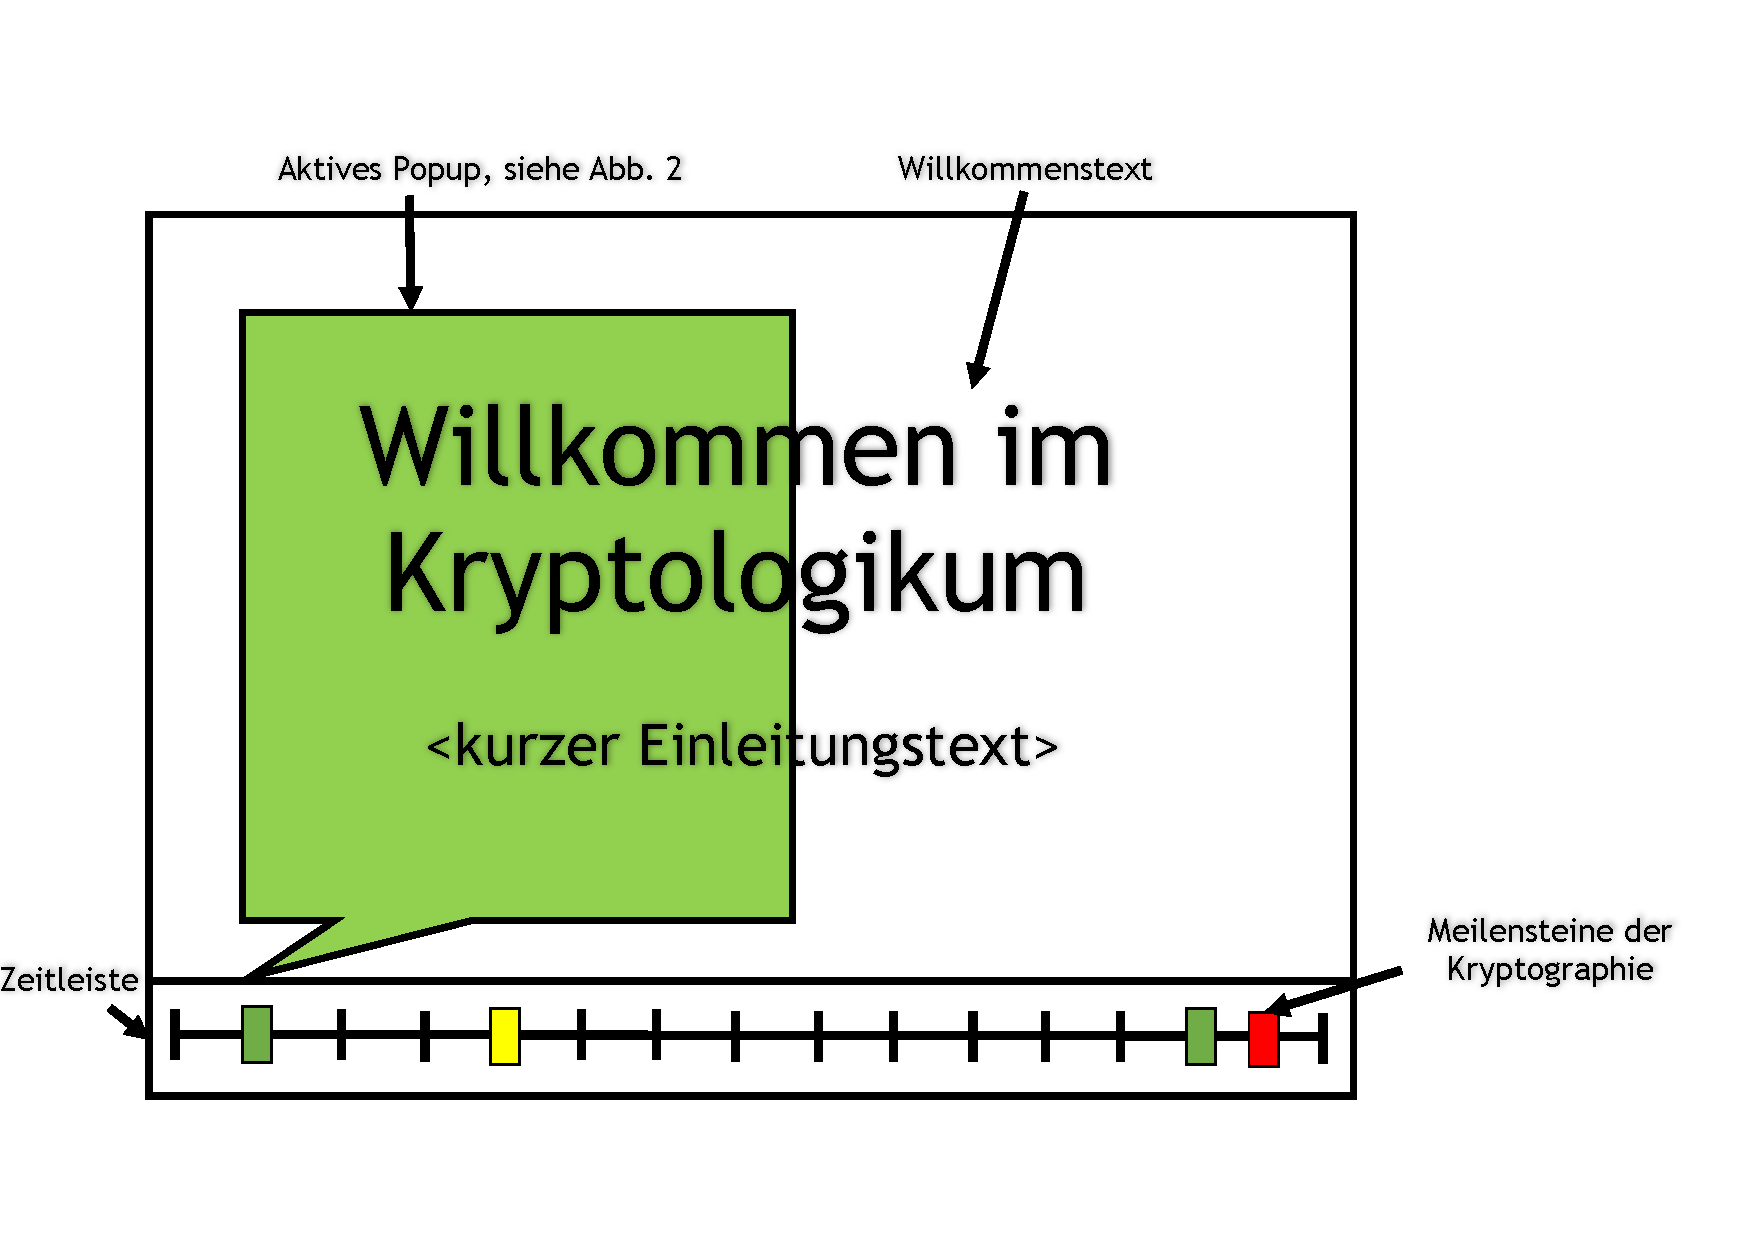
\includegraphics[width=\textwidth]{resources/ui_walkthrough_start-draft}
  \caption{Willkommensbildschirm mit Zeitleiste.}
\end{figure}

Sobald ein Meilenstein ausgewählt wurde, erscheint ein Popover (Fig. 2), dass den Namen, die Schwierigkeit und den Zweck des gewählten kryptografischen Verfahrens noch einmal zusammenfasst. Weiterhin werden ein Screenshot der eigentlichen Visualisierung sowie ein Button, um diese zu starten, dargestellt.

\begin{figure}[H]
  \centering
    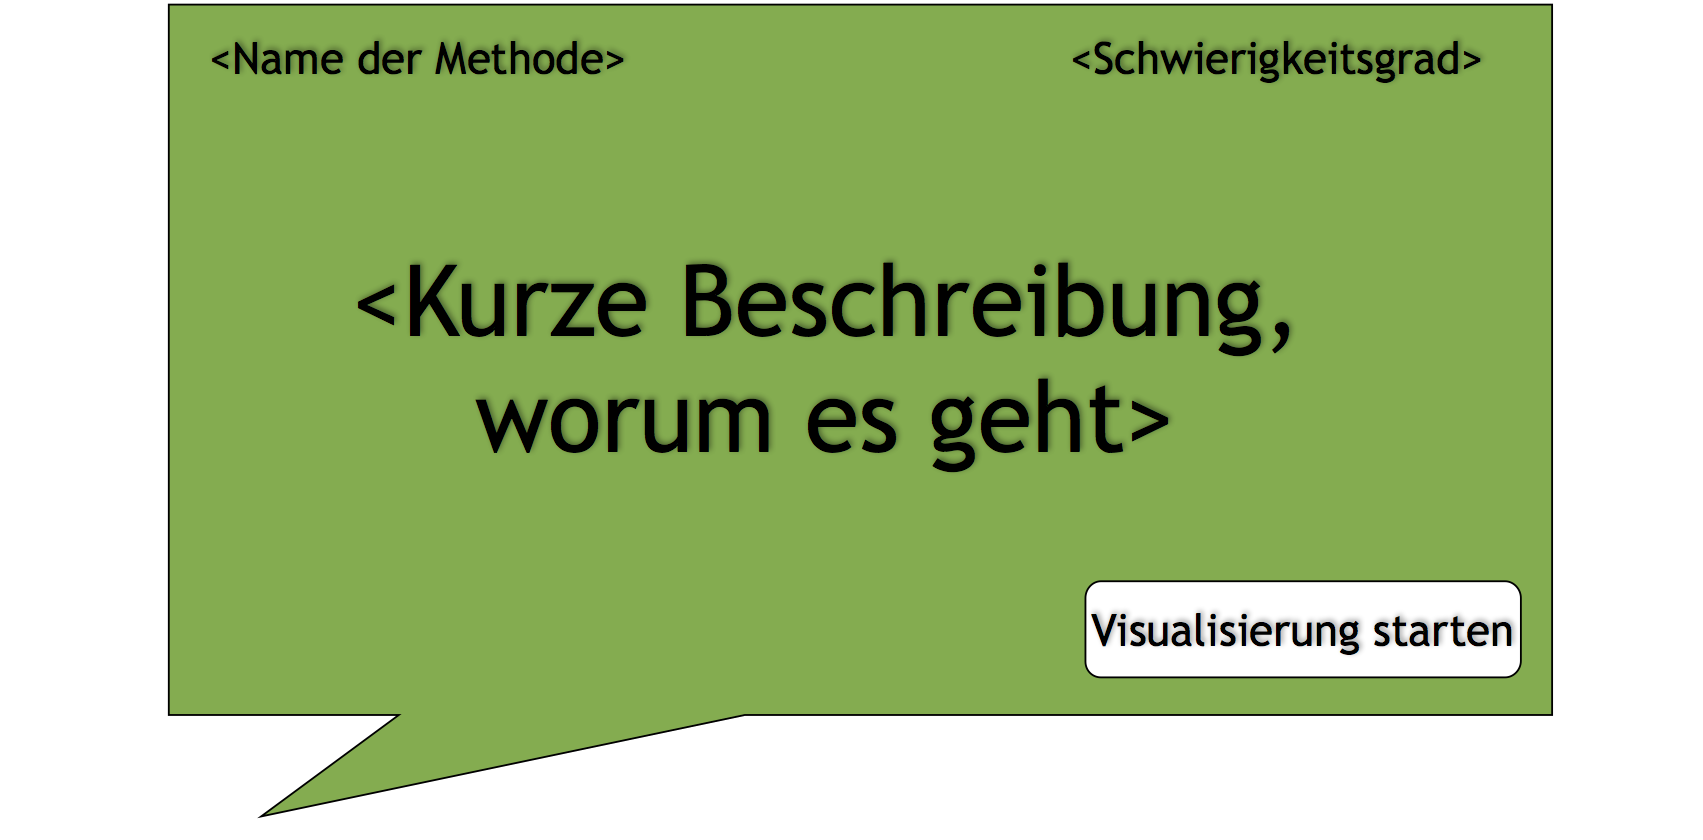
\includegraphics[width=\textwidth]{resources/ui_walkthrough_popover-draft}
  \caption{Detailansicht des Popovers in Fig. 1.}
\end{figure}

Nachdem der Benutzer eine Visualisierung startet, wird diese angezeigt (Fig. 3). Hierbei ist hervorzuheben, dass der Benutzer zu jedem Zeitpunkt die Visualisierung abbrechen kann, indem er auf den Button in der oberen linken Ecke klickt. Hilfe erhält er zu jedem Zeitpunkt im rechten oberen Eck.

\begin{figure}[H]
  \centering
    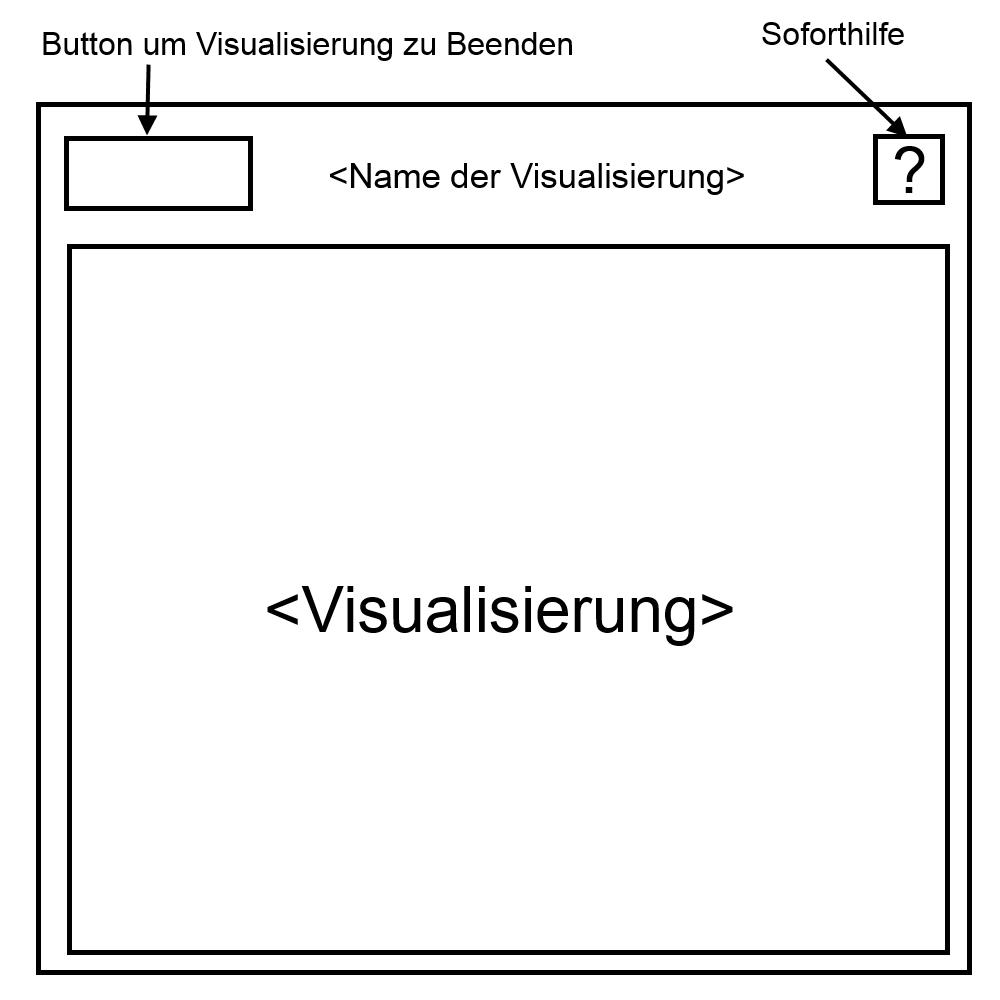
\includegraphics[width=\textwidth]{resources/ui_walkthrough_visualisation-draft}
  \caption{Darstellung einer Visualisierung.}
\end{figure}

Falls der Benutzer die Visualisierung erfolgreich beendet hat, wird (Fig 4.) angezeigt. Zunächst wird dem Benutzer zu seinem Erfolg gratuliert. Weiterhin besteht die prominente Möglichkeit, zum Willkommensbildschirm zurückzukehren. Falls das Interesse des Benutzers geweckt wurde, kann er sich weiterführendes Material mit nach Hause nehmen, indem er den abgebildeten QR-Code scant.

\begin{figure}[H]
  \centering
    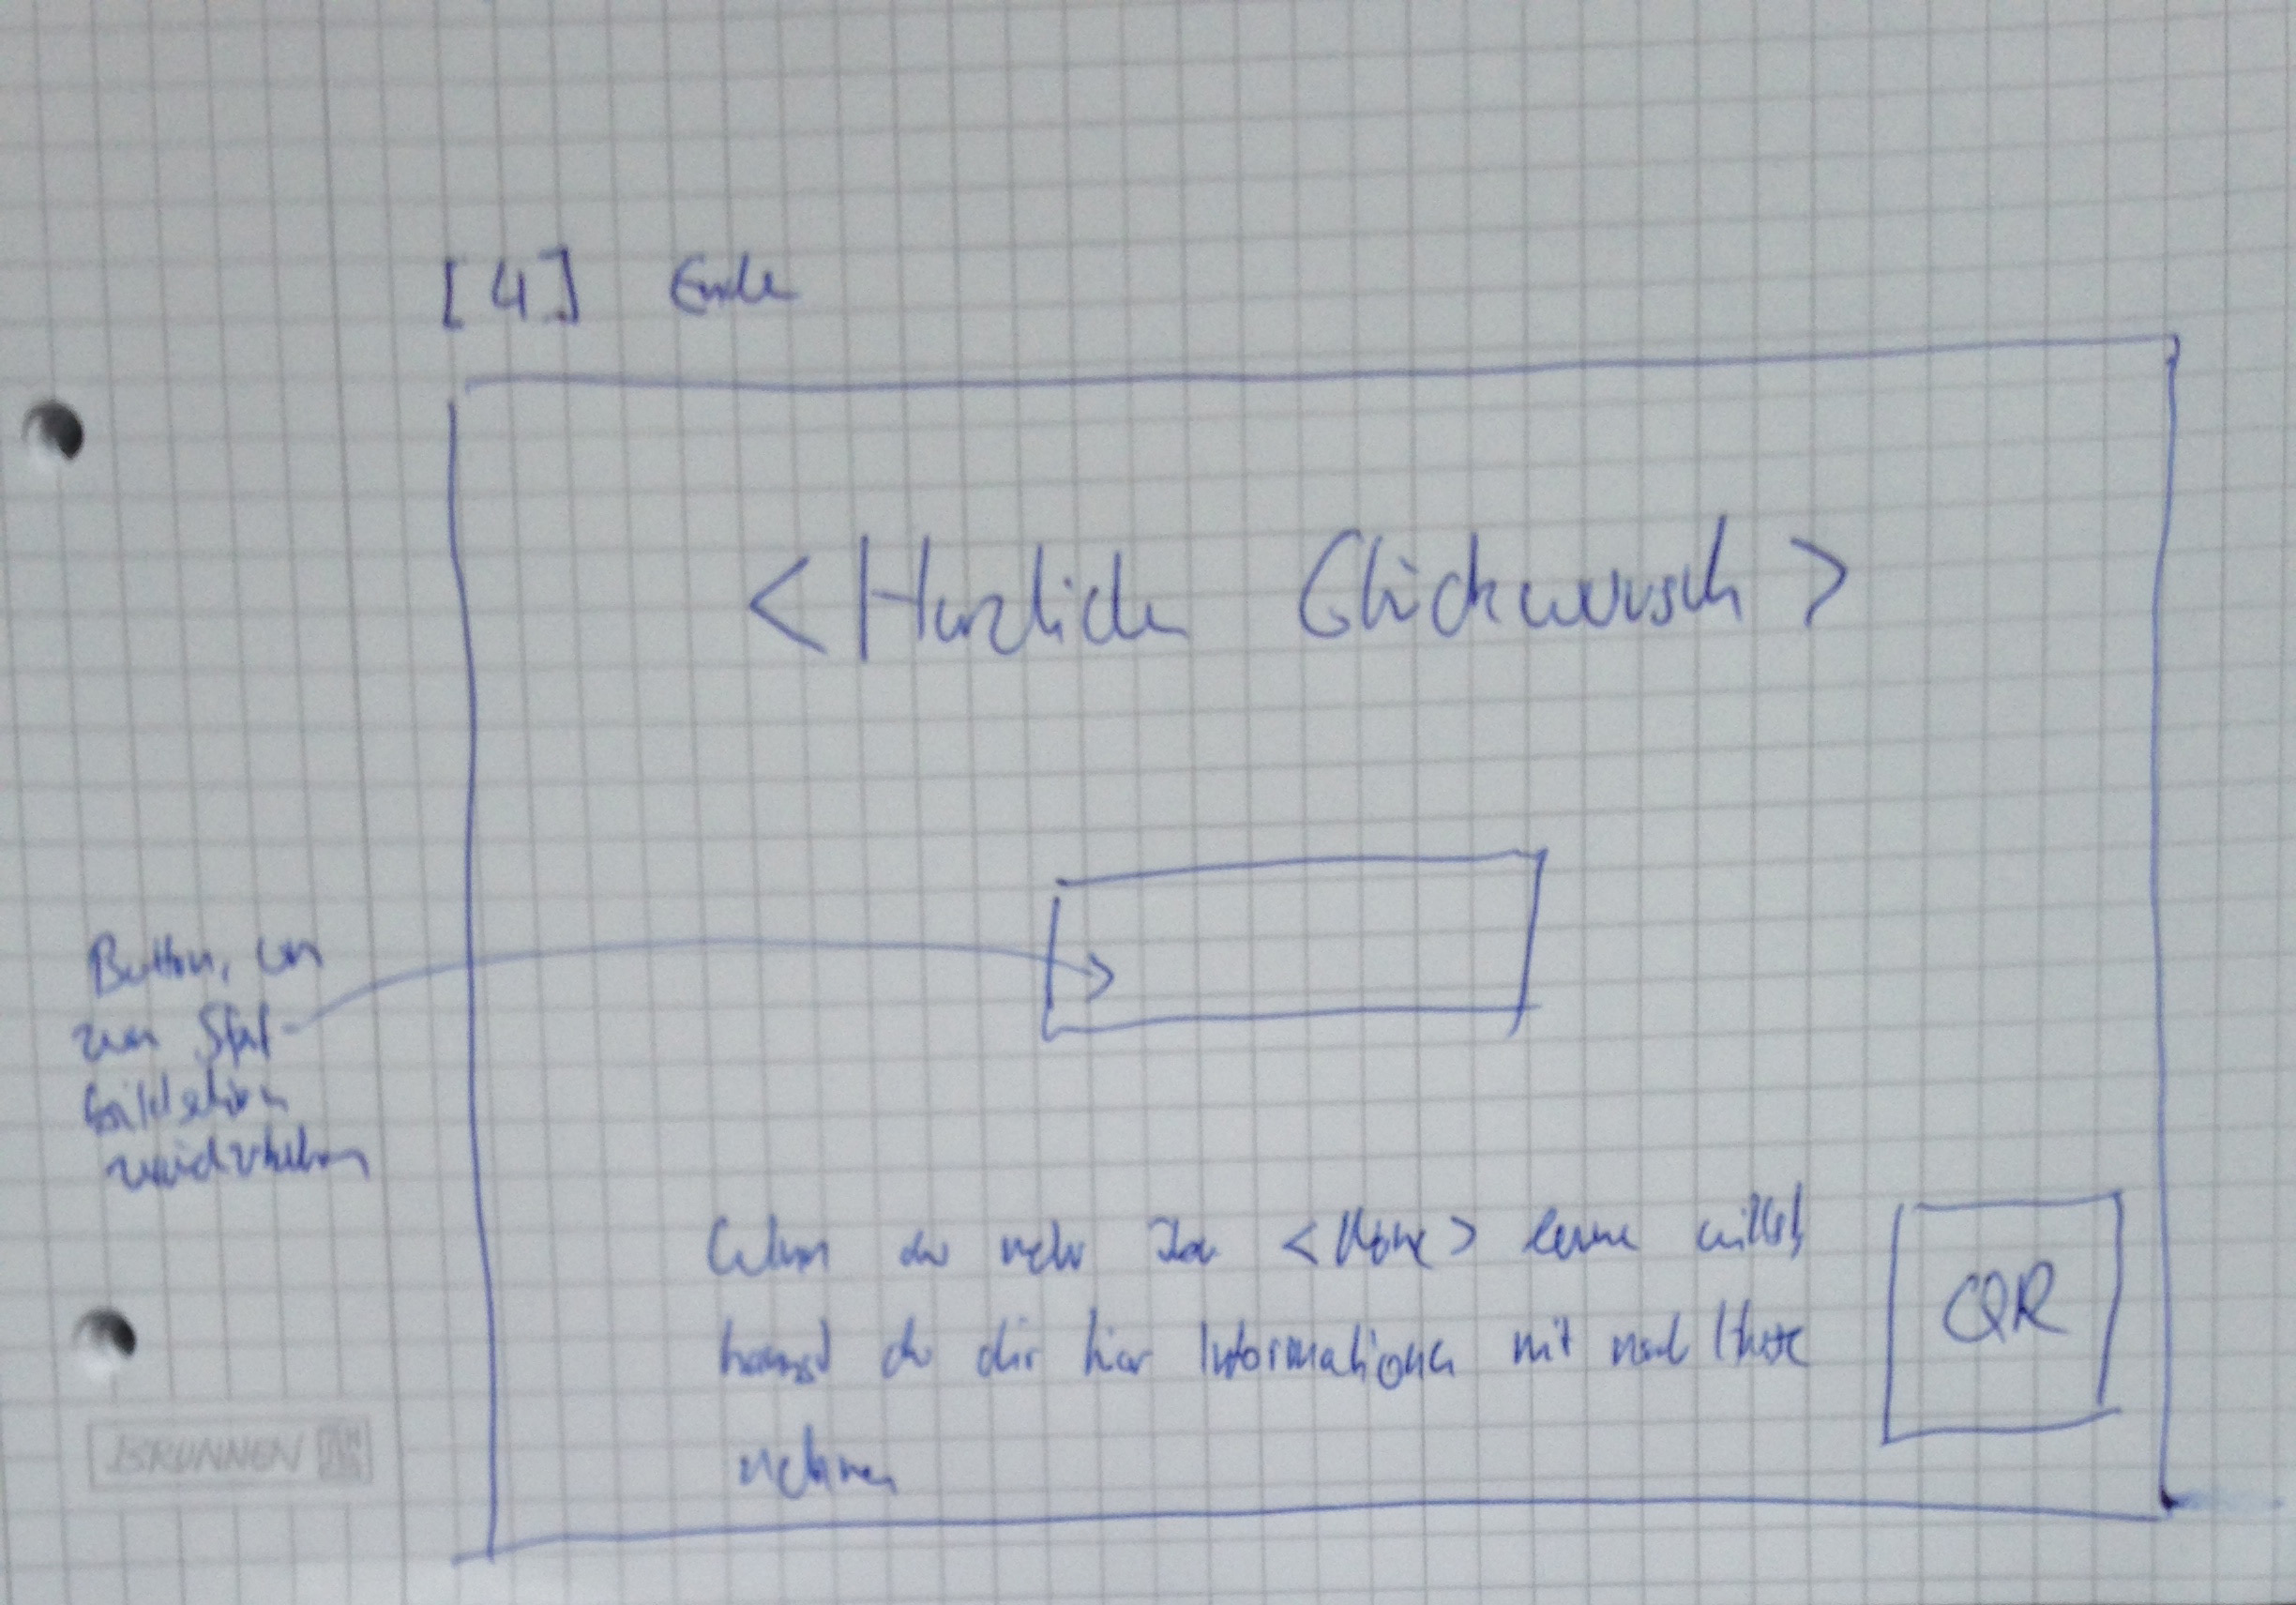
\includegraphics[width=\textwidth]{resources/ui_walkthrough_end-draft}
  \caption{Erfolgreiches Beenden einer Visualisierung.}
\end{figure}

\section{Globale Testfälle}
- automatisiertes Testen mithilfe von JUnit vor allem der Krypto-Algorithmen
- ggf. automatisiertes Testen der UI mithilfe von Szenarien und geeignetem Framework
Stresstest mit möglichst zufälligen und willkürlichen Eingaben (wie es Kinder eben tun)
Usability Tests mit passenden Testpersonen

\section{Systemmodelle}

\subsection{Systemübersicht}
Das System verwendet das bekannte MVC-Entwurfsmuster. Weiterhin ist geplant, das System in zwei Schichten zu unterteilen. Von unten nach oben enthält Schicht 1 wiederverendbare und in sich abgeschlossene Bibliotheken. Zum einen handelt es sich hierbei um Code von Dritten (z.B. um QR-Codes zu generieren). Weiterhin ist eine Sammlung wiederverwendbarer Klassen (nachfolgen {\it CGKit} genannt) geplant. {\it CGKit} wird vor allem aus UI-Elemente bestehen, die für die Implementierung aller Visualisierungen wertvoll sind.

\begin{figure}[h!]
  \centering
    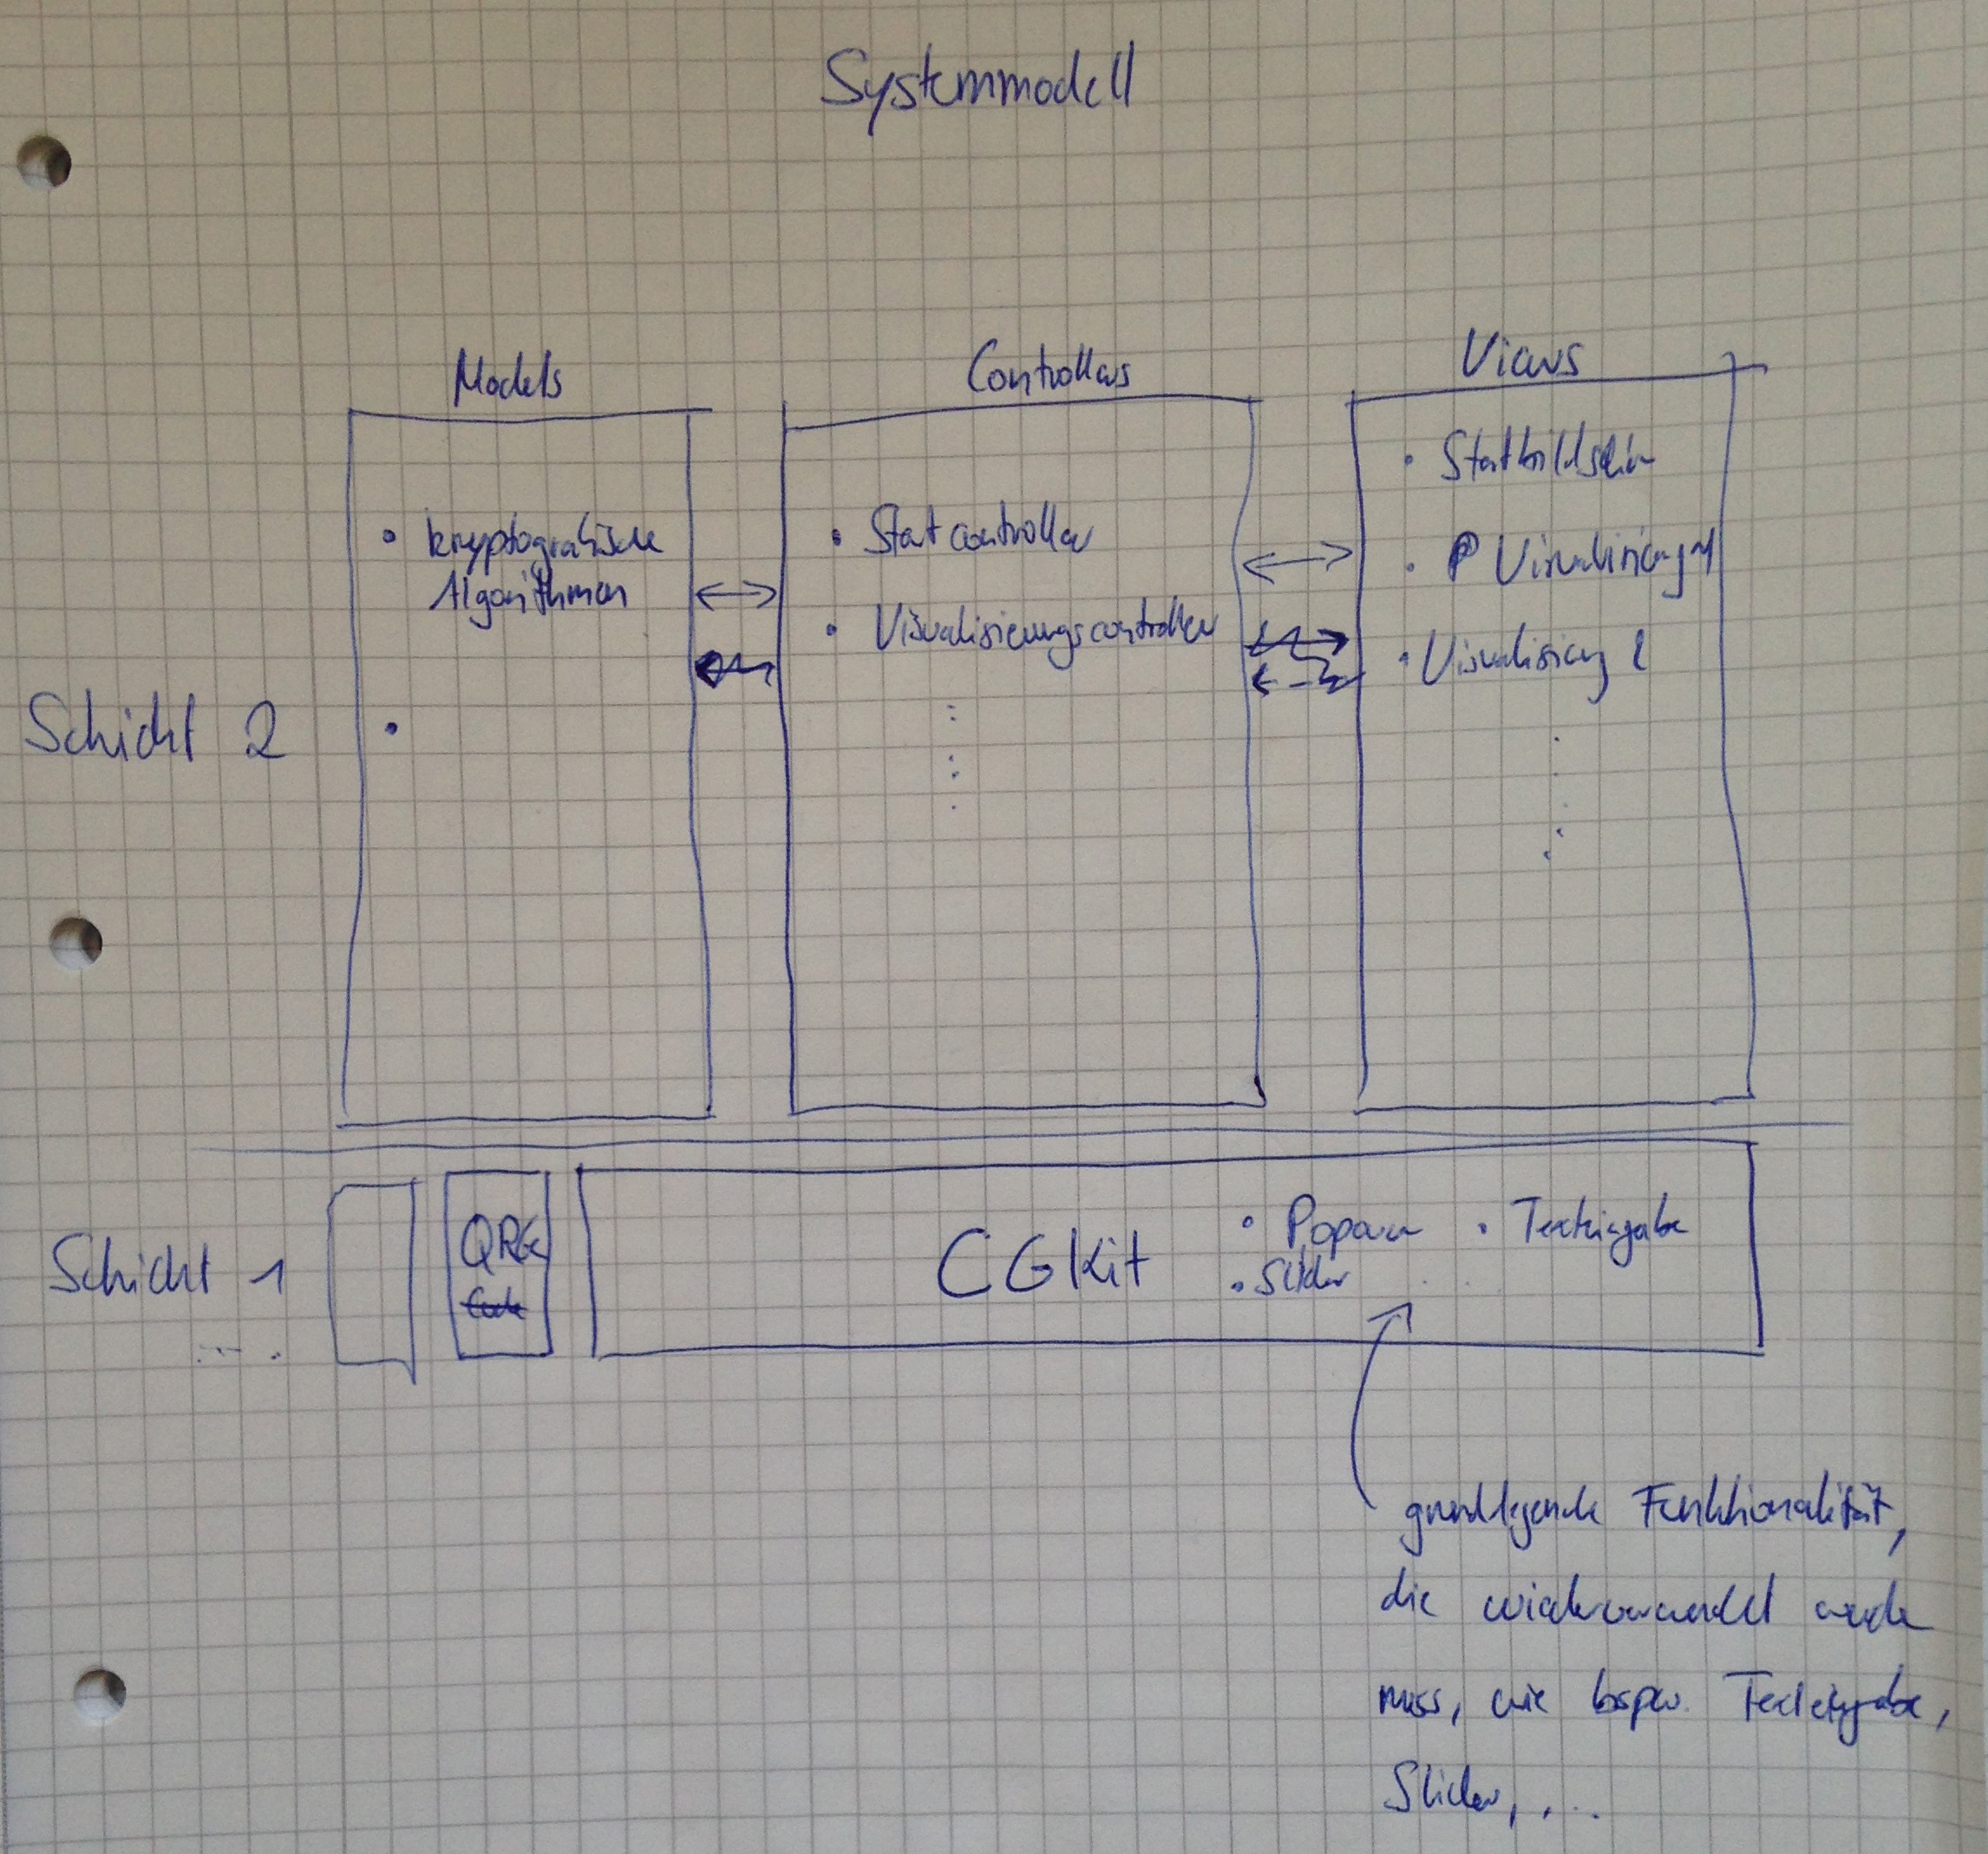
\includegraphics[width=\textwidth]{resources/systemmodel-draft}
  \caption{Schematische Darstellung des beschriebenen Systems.}
\end{figure}

\section{Beispielszenarien}
\begin{itemize}
    \item Beispiel läuft schrittweise ab. Problem wird dargestellt: A möchte B eine Nachricht schicken, die nicht von einer anderen Person als B gelesen werden soll. C versucht die Nachricht zu bekommen. Dabei können A und B nur über ein unsicheres Medium kommunizieren (Analogie z.B. schlüssel per Post verschicken), das von C abgehört wird.
itemA und B generieren ihre Schlüsselpaare. Der genaue Schlüssel ist nicht relevant.
\item A fragt B nach seinem public key, den B auch bereitwillig mitteilt. C hört den public key von B.
\item A verschlüsselt die Nachricht mit dem public key von B und verschickt die Nachricht an B. C hört die verschlüsselte Nachricht ab.
\item B entschlüsselt die Nachricht von A mit seinem private key und kann die Nachricht lesen
\item C versucht mit der Nachricht irgendetwas anzufangen und versucht sie mit dem abgehörten public key von B zu entschlüsseln. Das scheitert natürlich.

Beispiel einer Visualisierung anhand des Caesar-Algos:

\item Es wird erklärt, dass vermutlich Caesar dieses Verfahren verwendet hat um geheime Nachrichten zu verschlüsseln
\item Erklärung des Prinzips an einem Beispielsatz. Es werden schrittweise alle gleichen Buchstaben markiert und in ihr Äquivalent umgewandelt (z.B. "Hallo, wie geht's?" -> zuerst alle H zu K, dann alle a zu d, dann alle l zu o). Hier gibt es die Möglichkeit, schrittweise durchzugehen und noch mal zurück zu gehen. Außerdem kann man wenn man das Prinzip verstanden hat ans Ende springen.
\item Als nächstes muss die Person ein Wort selbst verschlüsseln mit Vorschrift (z.B. a -> b).
\item Am Ende wird mithilfe eines Diagrammes und der Kenntnis, das E der häufigste Buchstabe im Deutschen ist gezeigt, dass man diese Verschlüsselung leicht umgehen kann
\end{itemize}

\textbf{Szenario 1}:
Bob ist interessiert in Kryptographie und besucht zu diesem Anlass das Kryptologikum, um mehr Informationen diesbezüglich zu erhalten. Er nähert sich dem Cryptographics, wo ein Bildschirmschoner verschiedene kryptographische Verfahren Teaser-ähnlich visualisiert. Eine Berührung des Bildschirmes zeigt die Willkommensoberfläche von Cryptographics: Ein Zeitstrahl, auf dem chronologisch angeordnet verschiedene kryptographische Verfahren, ihrem Erfindungsjahr zugeordnet, genannt werden und farblich durch ihre Komplexität von grün (leicht) bis rot (schwer) gekennzeichnet sind. Bob wählt durch eine Berührung die Cäsar-Chiffre aus, sie befindet sich nämlich ganz am Anfang des Zeitstrahls. Daraufhin erscheint eine kurze Einleitung als Popup, im Hintergrund baut sich die Oberfläche auf und der Zeitstrahl gleitet verkleinert als Gesamtübersicht an den unteren Bildschirmrand. Nach dem Durchlesen der Einleitung schließt Bob das Popup, und er sieht eine Demonstration der Cäsar-Chiffre als Schritt-für-Schritt-Beispiel auf einer speziell für das Verfahren ausgelegten Oberfläche. Auf genau dieser Oberfläche kann Bob nach dem Beispiel sein neu erlerntes Wissen über das Verfahren anwenden, um Texte zu verschlüsseln, und durch einen gegebenen Schlüssel zu entschlüsseln. Nachdem er das Verfahren nun verinnerlicht hat, kann Bob das nächste Verfahren auswählen, entweder durch Drücken der “Weiter”-Taste, oder indem er ein Verfahren direkt am Zeitstrahl auswählt. Da er die weiteren Verfahren auch noch sehen möchte, arbeitet er sich am Zeitstrahl entlang durch das Programm, wobei er dann schließlich auf das Diffie-Hellman-Verfahren trifft, über welches er noch mehr Informationen erhalten möchte. Er berührt einen dafür vorgesehenen Button, welcher ein Popup mit einem QR-Code öffnet, dass letztendlich zu den ausführlichen Quellen weiterleitet. Alternativ ist dort auch eine gekürzte URL zu finden die man schnell abschreiben kann (Bsp.: http://goo.gl/abcd12).

\textbf{Szenario 2}:
Die ungeduldige Alice wurde von ihrer Freundin überredet, an der Ausstellung teilzunehmen. Sie sieht das Cryptographics und versucht, es durch wiederholte zufällige Eingaben zum Absturz zu bringen. Das Programm zeigt sich jedoch schnell als zu robust, um einem solchen Angriff zu erliegen. Schließlich wählt sie das komplizierteste kryptographische Verfahren aus, um Besuchern nach ihr den Einstieg zu erschweren. Nachdem sie gegangen ist, muss sie jedoch enttäuscht feststellen, dass der nächste Besucher keine weitere Schwierigkeiten hatte, das Programm mit dem dafür vorgesehenen Button in den Grundzustand zurückzuversetzen.

\textbf{Szenario 3}:
Nachdem Bob nun längere Zeit an Cryptographics verbracht hat, blickt er erschreckt auf die Uhr um festzustellen, dass es schon viel zu spät geworden ist. Er bricht auf, und lässt das Programm genau so zurück, wie er es gerade eben noch benutzt hat. x Sekunden nach seiner letzten Interaktion erscheint eine Meldung, die Bob darauf hingewiesen hätte, dass sich das Programm bald zurücksetzt, sollte in den nächsten y Sekunden keine Eingabe mehr erfolgen. Da er jedoch schon an der Bushaltestelle steht, aktiviert Cryptographics nun den Bildschirmschoner, den Bob zuvor auch schon vorgefunden hatte, und setzt im Hintergrund das Programm wieder auf den Ursprungszustand zurück.

\textbf{Szenario 4}:
Die Ausstellung ist für diesen Tag nun zu Ende, und die Kryptologikum-Administratorin Claudia schließt gerade noch die Tür hinter Bob ab, um sich jetzt den strombetriebenen Exponaten zu widmen. Als sie am Cryptographics ankommt, versucht sie zunächst, irgendwie zum Betriebssystem zurückzukehren, um den PC sicher herunterfahren zu können. Nach kurzer Zeit stellt sie fest, dass das ohne eine zusätzlich eingesteckte Hardware-Tastatur auf keinen Fall möglich ist. Sie holt also eine USB-Tastatur, steckt sie ein, kehrt über den Windows-Taskmanager zum Betriebssystem zurück, fährt den PC herunter und macht die Lichter aus.

\begin{figure}[h!]
  \centering
    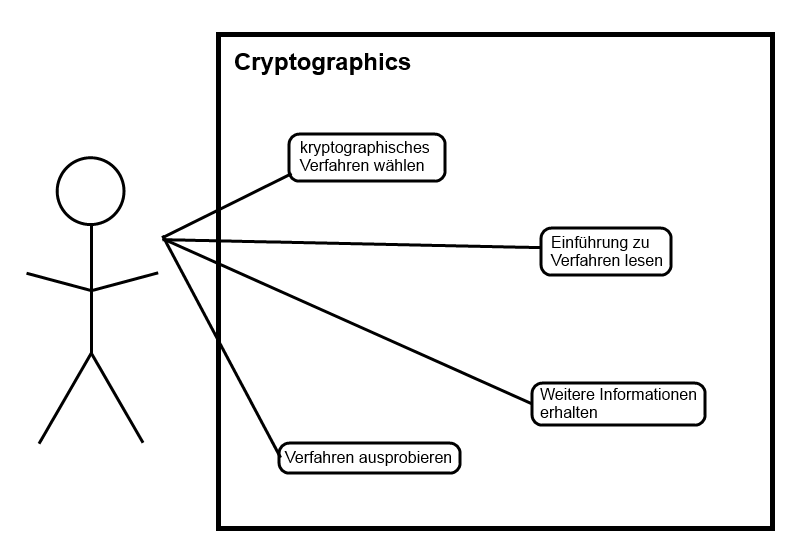
\includegraphics[width=\textwidth]{resources/usecase1}
  \caption{Anwendungsfalldiagramm zu beschriebenen Szenarien.}
\end{figure}

\section{Qualitätsbestimmung}

\end{document}


